
Let $x$ and $y$ be number of dolls of type $A$ and $B$ respectively such that 
\begin{align}
    x \geq 0 \\
    y \geq 0 
\end{align}
According to the question,
\begin{align}
    x+y &\leq 1200 
\end{align}
\begin{align}
   x-3y &\leq 600 
\end{align}
\begin{align}
-x+2y&\leq 0
\end{align}
$\therefore$ 
\begin{align}
        \max_{\vec{x}} Z &= \myvec{12 & 16}\vec{x}
\end{align}
$\therefore$ Our problem is
\begin{align}
        \max_{\vec{x}} Z &= \myvec{12 & 16}\vec{x}\\
        s.t. \quad 
        \myvec{1 & 1 \\ 1 & -3 \\ -1 & 2 }\vec{x} &\preceq \myvec{1200\\600\\0}
\end{align}

Lagrangian function is given by
\begin{equation}
\begin{aligned}
    &L(\vec{x},\boldsymbol{\lambda}) \\ &= \myvec{12 & 16}\vec{x}+\lcbrak{\sbrak{\myvec{1 & 1}\vec{x}-1200}} \\ &+ \sbrak{\myvec{1 & -3}\vec{x}-600} +\sbrak{\myvec{-1 & 2}\vec{x}} \\ &+ \sbrak{\myvec{-1 & 0}\vec{x}} +\rcbrak{\sbrak{\myvec{0 & -1}\vec{x}}}\boldsymbol{\lambda}
\end{aligned}
\end{equation}
where,
\begin{align}
    \boldsymbol{\lambda} &= \myvec{\lambda_1 \\ \lambda_2 \\ \lambda_3 \\ \lambda_4 \\ \lambda_5 \\ \lambda_6}
\end{align}

Now,
\begin{align}
    \nabla L(\vec{x},\boldsymbol{\lambda}) &= \myvec{12+ \myvec{1 & 1 & 2 & -1 & 0 }\boldsymbol{\lambda}\\ 16+\myvec{1 & -3 & -1 & 0 & -1}\boldsymbol{\lambda} \\ \myvec{1 & 1}\vec{x}-1200 \\ \myvec{-1 & -3}\vec{x}-600 \\ \myvec{-1 & 2}\vec{x}\\ \myvec{-1 & 0}\vec{x} \\ \myvec{0 & -1}\vec{x}}
\end{align}

$\therefore$ Lagrangian matrix is given by
\begin{align}
    \myvec{0 & 0 & 1 & 1 & 2 & -1 & 0 \\ 0 & 0 & 1 & -3 & -1 & 0 & -1 \\ 1 & 1 & 0 & 0 & 0 & 0 & 0 \\ 1 & -3 & 0 & 0 & 0 & 0 & 0 \\ -1 & 2 & 0 & 0 & 0 & 0 & 0 \\ -1 & 0 & 0 & 0 & 0 & 0 & 0 \\ 0 & -1 & 0 & 0 & 0 & 0 & 0 }\myvec{\vec{x} \\ \boldsymbol{\lambda} } &= \myvec{-12 \\ -16 \\ 1200 \\ 600 \\ 0 \\ 0 \\0 }
\end{align}
Considering $\lambda_1,\lambda_2$ as only active multiplier,
\begin{align}
    \myvec{0 & 0 & 1 & 2 \\ 0 & 0 & 1 & -1 \\ 1 & 1 & 0 & 0 \\ -1 & 2 & 0 & 0}\myvec{\vec{x}\\ \boldsymbol{\lambda}} &= \myvec{-12 \\ -16 \\ 1200 \\ 0}
\end{align}
resulting in,
\begin{align}
    \myvec{\vec{x} \\ \boldsymbol{\lambda}} &= \myvec{0 & 0 & 1 & 2 \\ 0 & 0 & 1 & -1 \\ 1 & 1 & 0 & 0 \\ -1 & 2 & 0 & 0}^{-1}\myvec{-12 \\ -16 \\ 1200 \\ 0}
    \\
    \implies   \myvec{\vec{x} \\ \boldsymbol{\lambda}} &= \myvec{0 & 0 & \frac{2}{3} & \frac{-1}{3} \\ 0 & 0 & \frac{1}{3} & \frac{1}{3} \\ \frac{1}{3} & \frac{2}{3} & 0 & 0 \\ \frac{1}{3} & \frac{-1}{3} & 0 & 0}\myvec{-12 \\ -16 \\ 1200 \\ 0}
    \\
    \implies \myvec{\vec{x} \\ \boldsymbol{\lambda}} &= \myvec{800 \\ 400 \\ \frac{-44}{3} \\ \frac{4}{3} }
\end{align}
$\because \boldsymbol{\lambda}=\myvec{\frac{-44}{3} \\ \frac{4}{3}} \succ \vec{0}$ 
\\
$\therefore$ Optimal solution is given by
\begin{align}
    \vec{x} &= \myvec{800\\400} \\
    Z &= \myvec{12 & 16}\vec{x} \\
    &= \myvec{12 & 16}\myvec{800 \\ 400} \\
    &= 16000
\end{align}
By using cvxpy in python ,
\begin{align}
    \vec{x}=\myvec{800.00001236\\399.99998704}\\
    Z = 15999.99994089
\end{align}
Hence ,the profit will be maximum if company produces.
Type A dolls = \boxed{800},
Type B dolls = \boxed{400}.
This is verified in Fig. \ref{opt/32/fig:TOY PROBLEM}.	
\begin{figure}[!ht]
\centering
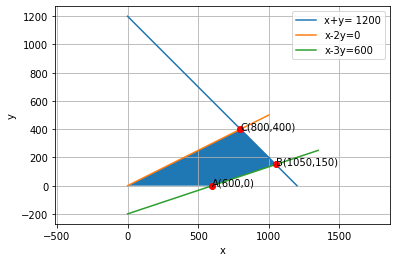
\includegraphics[width=\columnwidth]{solutions/su2021/2/32/download.png}
\caption{TOY PROBLEM}
\label{opt/32/fig:TOY PROBLEM}	
\end{figure}

